% Digital Logic Report Template
% Created: 2020-01-10, John Miller

%==========================================================
%=========== Document Setup  ==============================

% Formatting defined by class file
\documentclass[11pt]{article}

% ---- Document formatting ----
\usepackage[margin=1in]{geometry}	% Narrower margins
\usepackage{booktabs}				% Nice formatting of tables
\usepackage{graphicx}				% Ability to include graphics

%\setlength\parindent{0pt}	% Do not indent first line of paragraphs 
\usepackage[parfill]{parskip}		% Line space b/w paragraphs
%	parfill option prevents last line of pgrph from being fully justified

% Parskip package adds too much space around titles, fix with this
\RequirePackage{titlesec}
\titlespacing\section{0pt}{8pt plus 4pt minus 2pt}{3pt plus 2pt minus 2pt}
\titlespacing\subsection{0pt}{4pt plus 4pt minus 2pt}{-2pt plus 2pt minus 2pt}
\titlespacing\subsubsection{0pt}{2pt plus 4pt minus 2pt}{-6pt plus 2pt minus 2pt}

% ---- Hyperlinks ----
\usepackage[colorlinks=true,urlcolor=blue]{hyperref}	% For URL's. Automatically links internal references.

% ---- Code listings ----
\usepackage{listings} 					% Nice code layout and inclusion
\usepackage[usenames,dvipsnames]{xcolor}	% Colors (needs to be defined before using colors)

% Define custom colors for listings
\definecolor{listinggray}{gray}{0.98}		% Listings background color
\definecolor{rulegray}{gray}{0.7}			% Listings rule/frame color

% Style for Verilog
\lstdefinestyle{Verilog}{
	language=Verilog,					% Verilog
	backgroundcolor=\color{listinggray},	% light gray background
	rulecolor=\color{blue}, 			% blue frame lines
	frame=tb,							% lines above & below
	linewidth=\columnwidth, 			% set line width
	basicstyle=\small\ttfamily,	% basic font style that is used for the code	
	breaklines=true, 					% allow breaking across columns/pages
	tabsize=3,							% set tab size
	commentstyle=\color{gray},	% comments in italic 
	stringstyle=\upshape,				% strings are printed in normal font
	showspaces=false,					% don't underscore spaces
}

% How to use: \Verilog[listing_options]{file}
\newcommand{\Verilog}[2][]{%
	\lstinputlisting[style=Verilog,#1]{#2}
}




%======================================================
%=========== Body  ====================================
\begin{document}

\title{ELC 2137 Lab \#8: 4-digit Display}
\author{Sean Dickenscheidt and Sebastian Lopez}

\maketitle


\section*{Summary}

In this lab, using LaTeX and Git, it was discovered how to use and create tables. It was also learned how to use the Git program and uploading documents. Learned the basics of using LaTeX.






\section*{Results}

\begin{figure}[ht]\centering
	
	
	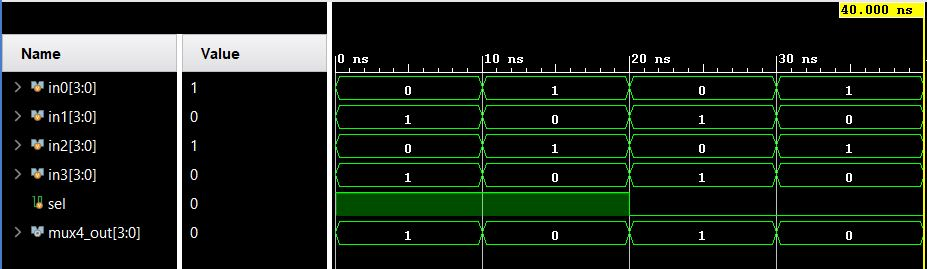
\includegraphics[width=1\textwidth]{mux4.JPG}
	\caption{mux4 ERT}
	\label{fig:sim_with_table}
	
\end{figure}
\begin{figure}[ht]\centering
	

	
	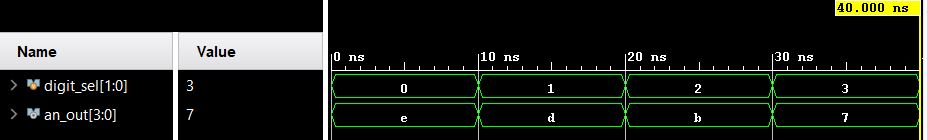
\includegraphics[width=1\textwidth]{an_test.JPG}
	\caption{an decoder ERT}
	\label{fig:sim_with_table}

\end{figure}


\clearpage
\section*{Code}

\begin{lstlisting}[style=Verilog,
caption=mux2 Code,
label=code:ex 
]
`timescale 1ns / 1ps
// ELC 2137 - Lab8 - 02/20/2020
// Sebastian Lopez and Sean Dickenscheidt
module mux2 #(parameter N = 2) (
input [N - 1:0] in0, in1,
input sel,
output [N - 1:0] mux2_out
); 

assign mux2_out = sel? in1:in0; 

endmodule  
\end{lstlisting}

\begin{lstlisting}[style=Verilog,
caption=mux4 Code,
label=code:ex 
]
`timescale 1ns / 1ps
// ELC 2137 - Lab8 - 02/20/2020
// Sebastian Lopez and Sean Dickenscheidt
module mux4 #(parameter N = 2) (
input [N - 1:0] in0, in1, in2, in3, 
input [1:0] sel, 
output reg [N - 1:0] mux4_out
);

always @*
case (sel) 
0: mux4_out <= in0; 
1: mux4_out <= in1; 
2: mux4_out <= in2; 
default: mux4_out <= in3;     
endcase 
endmodule //mux4 
\end{lstlisting}

\begin{lstlisting}[style=Verilog,
caption=an decoder Code,
label=code:ex 
]
`timescale 1ns / 1ps
// ELC 2137 - Lab8 - 02/20/2020
// Sebastian Lopez and Sean Dickenscheidt
module an_decoder (
input [1:0] digit_sel,
output reg [3:0] an_out
);

always @*
case (digit_sel) 
0: an_out <= 4'b1110; 
1: an_out <= 4'b1101; 
2: an_out <= 4'b1011; 
default: an_out <= 4'b0111;     
endcase 
endmodule //an_decoder 
\end{lstlisting}

\begin{lstlisting}[style=Verilog,
caption=sseg4 Code,
label=code:ex 
]
`timescale 1ns / 1ps
// ELC 2137 - Lab8 - 02/20/2020
// Sebastian Lopez and Sean Dickenscheidt
module sseg4 (
input [3:0] num,
output reg [6:0] sseg 
);

endmodule //sseg_decoder
\end{lstlisting}

\begin{lstlisting}[style=Verilog,
caption=sseg4 manual Code,
label=code:ex 
]
`timescale 1ns / 1ps
// ELC 2137 - Lab8 - 02/20/2020
// Sebastian Lopez and Sean Dickenscheidt
needs code 
\end{lstlisting}




\end{document}
